
% Default to the notebook output style

    


% Inherit from the specified cell style.




    
\documentclass[11pt]{article}

    
    
    \usepackage[T1]{fontenc}
    % Nicer default font (+ math font) than Computer Modern for most use cases
    \usepackage{mathpazo}

    % Basic figure setup, for now with no caption control since it's done
    % automatically by Pandoc (which extracts ![](path) syntax from Markdown).
    \usepackage{graphicx}
    % We will generate all images so they have a width \maxwidth. This means
    % that they will get their normal width if they fit onto the page, but
    % are scaled down if they would overflow the margins.
    \makeatletter
    \def\maxwidth{\ifdim\Gin@nat@width>\linewidth\linewidth
    \else\Gin@nat@width\fi}
    \makeatother
    \let\Oldincludegraphics\includegraphics
    % Set max figure width to be 80% of text width, for now hardcoded.
    \renewcommand{\includegraphics}[1]{\Oldincludegraphics[width=.8\maxwidth]{#1}}
    % Ensure that by default, figures have no caption (until we provide a
    % proper Figure object with a Caption API and a way to capture that
    % in the conversion process - todo).
    \usepackage{caption}
    \DeclareCaptionLabelFormat{nolabel}{}
    \captionsetup{labelformat=nolabel}

    \usepackage{adjustbox} % Used to constrain images to a maximum size 
    \usepackage{xcolor} % Allow colors to be defined
    \usepackage{enumerate} % Needed for markdown enumerations to work
    \usepackage{geometry} % Used to adjust the document margins
    \usepackage{amsmath} % Equations
    \usepackage{amssymb} % Equations
    \usepackage{textcomp} % defines textquotesingle
    % Hack from http://tex.stackexchange.com/a/47451/13684:
    \AtBeginDocument{%
        \def\PYZsq{\textquotesingle}% Upright quotes in Pygmentized code
    }
    \usepackage{upquote} % Upright quotes for verbatim code
    \usepackage{eurosym} % defines \euro
    \usepackage[mathletters]{ucs} % Extended unicode (utf-8) support
    \usepackage[utf8x]{inputenc} % Allow utf-8 characters in the tex document
    \usepackage{fancyvrb} % verbatim replacement that allows latex
    \usepackage{grffile} % extends the file name processing of package graphics 
                         % to support a larger range 
    % The hyperref package gives us a pdf with properly built
    % internal navigation ('pdf bookmarks' for the table of contents,
    % internal cross-reference links, web links for URLs, etc.)
    \usepackage{hyperref}
    \usepackage{longtable} % longtable support required by pandoc >1.10
    \usepackage{booktabs}  % table support for pandoc > 1.12.2
    \usepackage[inline]{enumitem} % IRkernel/repr support (it uses the enumerate* environment)
    \usepackage[normalem]{ulem} % ulem is needed to support strikethroughs (\sout)
                                % normalem makes italics be italics, not underlines
    

    
    
    % Colors for the hyperref package
    \definecolor{urlcolor}{rgb}{0,.145,.698}
    \definecolor{linkcolor}{rgb}{.71,0.21,0.01}
    \definecolor{citecolor}{rgb}{.12,.54,.11}

    % ANSI colors
    \definecolor{ansi-black}{HTML}{3E424D}
    \definecolor{ansi-black-intense}{HTML}{282C36}
    \definecolor{ansi-red}{HTML}{E75C58}
    \definecolor{ansi-red-intense}{HTML}{B22B31}
    \definecolor{ansi-green}{HTML}{00A250}
    \definecolor{ansi-green-intense}{HTML}{007427}
    \definecolor{ansi-yellow}{HTML}{DDB62B}
    \definecolor{ansi-yellow-intense}{HTML}{B27D12}
    \definecolor{ansi-blue}{HTML}{208FFB}
    \definecolor{ansi-blue-intense}{HTML}{0065CA}
    \definecolor{ansi-magenta}{HTML}{D160C4}
    \definecolor{ansi-magenta-intense}{HTML}{A03196}
    \definecolor{ansi-cyan}{HTML}{60C6C8}
    \definecolor{ansi-cyan-intense}{HTML}{258F8F}
    \definecolor{ansi-white}{HTML}{C5C1B4}
    \definecolor{ansi-white-intense}{HTML}{A1A6B2}

    % commands and environments needed by pandoc snippets
    % extracted from the output of `pandoc -s`
    \providecommand{\tightlist}{%
      \setlength{\itemsep}{0pt}\setlength{\parskip}{0pt}}
    \DefineVerbatimEnvironment{Highlighting}{Verbatim}{commandchars=\\\{\}}
    % Add ',fontsize=\small' for more characters per line
    \newenvironment{Shaded}{}{}
    \newcommand{\KeywordTok}[1]{\textcolor[rgb]{0.00,0.44,0.13}{\textbf{{#1}}}}
    \newcommand{\DataTypeTok}[1]{\textcolor[rgb]{0.56,0.13,0.00}{{#1}}}
    \newcommand{\DecValTok}[1]{\textcolor[rgb]{0.25,0.63,0.44}{{#1}}}
    \newcommand{\BaseNTok}[1]{\textcolor[rgb]{0.25,0.63,0.44}{{#1}}}
    \newcommand{\FloatTok}[1]{\textcolor[rgb]{0.25,0.63,0.44}{{#1}}}
    \newcommand{\CharTok}[1]{\textcolor[rgb]{0.25,0.44,0.63}{{#1}}}
    \newcommand{\StringTok}[1]{\textcolor[rgb]{0.25,0.44,0.63}{{#1}}}
    \newcommand{\CommentTok}[1]{\textcolor[rgb]{0.38,0.63,0.69}{\textit{{#1}}}}
    \newcommand{\OtherTok}[1]{\textcolor[rgb]{0.00,0.44,0.13}{{#1}}}
    \newcommand{\AlertTok}[1]{\textcolor[rgb]{1.00,0.00,0.00}{\textbf{{#1}}}}
    \newcommand{\FunctionTok}[1]{\textcolor[rgb]{0.02,0.16,0.49}{{#1}}}
    \newcommand{\RegionMarkerTok}[1]{{#1}}
    \newcommand{\ErrorTok}[1]{\textcolor[rgb]{1.00,0.00,0.00}{\textbf{{#1}}}}
    \newcommand{\NormalTok}[1]{{#1}}
    
    % Additional commands for more recent versions of Pandoc
    \newcommand{\ConstantTok}[1]{\textcolor[rgb]{0.53,0.00,0.00}{{#1}}}
    \newcommand{\SpecialCharTok}[1]{\textcolor[rgb]{0.25,0.44,0.63}{{#1}}}
    \newcommand{\VerbatimStringTok}[1]{\textcolor[rgb]{0.25,0.44,0.63}{{#1}}}
    \newcommand{\SpecialStringTok}[1]{\textcolor[rgb]{0.73,0.40,0.53}{{#1}}}
    \newcommand{\ImportTok}[1]{{#1}}
    \newcommand{\DocumentationTok}[1]{\textcolor[rgb]{0.73,0.13,0.13}{\textit{{#1}}}}
    \newcommand{\AnnotationTok}[1]{\textcolor[rgb]{0.38,0.63,0.69}{\textbf{\textit{{#1}}}}}
    \newcommand{\CommentVarTok}[1]{\textcolor[rgb]{0.38,0.63,0.69}{\textbf{\textit{{#1}}}}}
    \newcommand{\VariableTok}[1]{\textcolor[rgb]{0.10,0.09,0.49}{{#1}}}
    \newcommand{\ControlFlowTok}[1]{\textcolor[rgb]{0.00,0.44,0.13}{\textbf{{#1}}}}
    \newcommand{\OperatorTok}[1]{\textcolor[rgb]{0.40,0.40,0.40}{{#1}}}
    \newcommand{\BuiltInTok}[1]{{#1}}
    \newcommand{\ExtensionTok}[1]{{#1}}
    \newcommand{\PreprocessorTok}[1]{\textcolor[rgb]{0.74,0.48,0.00}{{#1}}}
    \newcommand{\AttributeTok}[1]{\textcolor[rgb]{0.49,0.56,0.16}{{#1}}}
    \newcommand{\InformationTok}[1]{\textcolor[rgb]{0.38,0.63,0.69}{\textbf{\textit{{#1}}}}}
    \newcommand{\WarningTok}[1]{\textcolor[rgb]{0.38,0.63,0.69}{\textbf{\textit{{#1}}}}}
    
    
    % Define a nice break command that doesn't care if a line doesn't already
    % exist.
    \def\br{\hspace*{\fill} \\* }
    % Math Jax compatability definitions
    \def\gt{>}
    \def\lt{<}
    % Document parameters
    \title{Python\_101}
    
    
    

    % Pygments definitions
    
\makeatletter
\def\PY@reset{\let\PY@it=\relax \let\PY@bf=\relax%
    \let\PY@ul=\relax \let\PY@tc=\relax%
    \let\PY@bc=\relax \let\PY@ff=\relax}
\def\PY@tok#1{\csname PY@tok@#1\endcsname}
\def\PY@toks#1+{\ifx\relax#1\empty\else%
    \PY@tok{#1}\expandafter\PY@toks\fi}
\def\PY@do#1{\PY@bc{\PY@tc{\PY@ul{%
    \PY@it{\PY@bf{\PY@ff{#1}}}}}}}
\def\PY#1#2{\PY@reset\PY@toks#1+\relax+\PY@do{#2}}

\expandafter\def\csname PY@tok@w\endcsname{\def\PY@tc##1{\textcolor[rgb]{0.73,0.73,0.73}{##1}}}
\expandafter\def\csname PY@tok@c\endcsname{\let\PY@it=\textit\def\PY@tc##1{\textcolor[rgb]{0.25,0.50,0.50}{##1}}}
\expandafter\def\csname PY@tok@cp\endcsname{\def\PY@tc##1{\textcolor[rgb]{0.74,0.48,0.00}{##1}}}
\expandafter\def\csname PY@tok@k\endcsname{\let\PY@bf=\textbf\def\PY@tc##1{\textcolor[rgb]{0.00,0.50,0.00}{##1}}}
\expandafter\def\csname PY@tok@kp\endcsname{\def\PY@tc##1{\textcolor[rgb]{0.00,0.50,0.00}{##1}}}
\expandafter\def\csname PY@tok@kt\endcsname{\def\PY@tc##1{\textcolor[rgb]{0.69,0.00,0.25}{##1}}}
\expandafter\def\csname PY@tok@o\endcsname{\def\PY@tc##1{\textcolor[rgb]{0.40,0.40,0.40}{##1}}}
\expandafter\def\csname PY@tok@ow\endcsname{\let\PY@bf=\textbf\def\PY@tc##1{\textcolor[rgb]{0.67,0.13,1.00}{##1}}}
\expandafter\def\csname PY@tok@nb\endcsname{\def\PY@tc##1{\textcolor[rgb]{0.00,0.50,0.00}{##1}}}
\expandafter\def\csname PY@tok@nf\endcsname{\def\PY@tc##1{\textcolor[rgb]{0.00,0.00,1.00}{##1}}}
\expandafter\def\csname PY@tok@nc\endcsname{\let\PY@bf=\textbf\def\PY@tc##1{\textcolor[rgb]{0.00,0.00,1.00}{##1}}}
\expandafter\def\csname PY@tok@nn\endcsname{\let\PY@bf=\textbf\def\PY@tc##1{\textcolor[rgb]{0.00,0.00,1.00}{##1}}}
\expandafter\def\csname PY@tok@ne\endcsname{\let\PY@bf=\textbf\def\PY@tc##1{\textcolor[rgb]{0.82,0.25,0.23}{##1}}}
\expandafter\def\csname PY@tok@nv\endcsname{\def\PY@tc##1{\textcolor[rgb]{0.10,0.09,0.49}{##1}}}
\expandafter\def\csname PY@tok@no\endcsname{\def\PY@tc##1{\textcolor[rgb]{0.53,0.00,0.00}{##1}}}
\expandafter\def\csname PY@tok@nl\endcsname{\def\PY@tc##1{\textcolor[rgb]{0.63,0.63,0.00}{##1}}}
\expandafter\def\csname PY@tok@ni\endcsname{\let\PY@bf=\textbf\def\PY@tc##1{\textcolor[rgb]{0.60,0.60,0.60}{##1}}}
\expandafter\def\csname PY@tok@na\endcsname{\def\PY@tc##1{\textcolor[rgb]{0.49,0.56,0.16}{##1}}}
\expandafter\def\csname PY@tok@nt\endcsname{\let\PY@bf=\textbf\def\PY@tc##1{\textcolor[rgb]{0.00,0.50,0.00}{##1}}}
\expandafter\def\csname PY@tok@nd\endcsname{\def\PY@tc##1{\textcolor[rgb]{0.67,0.13,1.00}{##1}}}
\expandafter\def\csname PY@tok@s\endcsname{\def\PY@tc##1{\textcolor[rgb]{0.73,0.13,0.13}{##1}}}
\expandafter\def\csname PY@tok@sd\endcsname{\let\PY@it=\textit\def\PY@tc##1{\textcolor[rgb]{0.73,0.13,0.13}{##1}}}
\expandafter\def\csname PY@tok@si\endcsname{\let\PY@bf=\textbf\def\PY@tc##1{\textcolor[rgb]{0.73,0.40,0.53}{##1}}}
\expandafter\def\csname PY@tok@se\endcsname{\let\PY@bf=\textbf\def\PY@tc##1{\textcolor[rgb]{0.73,0.40,0.13}{##1}}}
\expandafter\def\csname PY@tok@sr\endcsname{\def\PY@tc##1{\textcolor[rgb]{0.73,0.40,0.53}{##1}}}
\expandafter\def\csname PY@tok@ss\endcsname{\def\PY@tc##1{\textcolor[rgb]{0.10,0.09,0.49}{##1}}}
\expandafter\def\csname PY@tok@sx\endcsname{\def\PY@tc##1{\textcolor[rgb]{0.00,0.50,0.00}{##1}}}
\expandafter\def\csname PY@tok@m\endcsname{\def\PY@tc##1{\textcolor[rgb]{0.40,0.40,0.40}{##1}}}
\expandafter\def\csname PY@tok@gh\endcsname{\let\PY@bf=\textbf\def\PY@tc##1{\textcolor[rgb]{0.00,0.00,0.50}{##1}}}
\expandafter\def\csname PY@tok@gu\endcsname{\let\PY@bf=\textbf\def\PY@tc##1{\textcolor[rgb]{0.50,0.00,0.50}{##1}}}
\expandafter\def\csname PY@tok@gd\endcsname{\def\PY@tc##1{\textcolor[rgb]{0.63,0.00,0.00}{##1}}}
\expandafter\def\csname PY@tok@gi\endcsname{\def\PY@tc##1{\textcolor[rgb]{0.00,0.63,0.00}{##1}}}
\expandafter\def\csname PY@tok@gr\endcsname{\def\PY@tc##1{\textcolor[rgb]{1.00,0.00,0.00}{##1}}}
\expandafter\def\csname PY@tok@ge\endcsname{\let\PY@it=\textit}
\expandafter\def\csname PY@tok@gs\endcsname{\let\PY@bf=\textbf}
\expandafter\def\csname PY@tok@gp\endcsname{\let\PY@bf=\textbf\def\PY@tc##1{\textcolor[rgb]{0.00,0.00,0.50}{##1}}}
\expandafter\def\csname PY@tok@go\endcsname{\def\PY@tc##1{\textcolor[rgb]{0.53,0.53,0.53}{##1}}}
\expandafter\def\csname PY@tok@gt\endcsname{\def\PY@tc##1{\textcolor[rgb]{0.00,0.27,0.87}{##1}}}
\expandafter\def\csname PY@tok@err\endcsname{\def\PY@bc##1{\setlength{\fboxsep}{0pt}\fcolorbox[rgb]{1.00,0.00,0.00}{1,1,1}{\strut ##1}}}
\expandafter\def\csname PY@tok@kc\endcsname{\let\PY@bf=\textbf\def\PY@tc##1{\textcolor[rgb]{0.00,0.50,0.00}{##1}}}
\expandafter\def\csname PY@tok@kd\endcsname{\let\PY@bf=\textbf\def\PY@tc##1{\textcolor[rgb]{0.00,0.50,0.00}{##1}}}
\expandafter\def\csname PY@tok@kn\endcsname{\let\PY@bf=\textbf\def\PY@tc##1{\textcolor[rgb]{0.00,0.50,0.00}{##1}}}
\expandafter\def\csname PY@tok@kr\endcsname{\let\PY@bf=\textbf\def\PY@tc##1{\textcolor[rgb]{0.00,0.50,0.00}{##1}}}
\expandafter\def\csname PY@tok@bp\endcsname{\def\PY@tc##1{\textcolor[rgb]{0.00,0.50,0.00}{##1}}}
\expandafter\def\csname PY@tok@fm\endcsname{\def\PY@tc##1{\textcolor[rgb]{0.00,0.00,1.00}{##1}}}
\expandafter\def\csname PY@tok@vc\endcsname{\def\PY@tc##1{\textcolor[rgb]{0.10,0.09,0.49}{##1}}}
\expandafter\def\csname PY@tok@vg\endcsname{\def\PY@tc##1{\textcolor[rgb]{0.10,0.09,0.49}{##1}}}
\expandafter\def\csname PY@tok@vi\endcsname{\def\PY@tc##1{\textcolor[rgb]{0.10,0.09,0.49}{##1}}}
\expandafter\def\csname PY@tok@vm\endcsname{\def\PY@tc##1{\textcolor[rgb]{0.10,0.09,0.49}{##1}}}
\expandafter\def\csname PY@tok@sa\endcsname{\def\PY@tc##1{\textcolor[rgb]{0.73,0.13,0.13}{##1}}}
\expandafter\def\csname PY@tok@sb\endcsname{\def\PY@tc##1{\textcolor[rgb]{0.73,0.13,0.13}{##1}}}
\expandafter\def\csname PY@tok@sc\endcsname{\def\PY@tc##1{\textcolor[rgb]{0.73,0.13,0.13}{##1}}}
\expandafter\def\csname PY@tok@dl\endcsname{\def\PY@tc##1{\textcolor[rgb]{0.73,0.13,0.13}{##1}}}
\expandafter\def\csname PY@tok@s2\endcsname{\def\PY@tc##1{\textcolor[rgb]{0.73,0.13,0.13}{##1}}}
\expandafter\def\csname PY@tok@sh\endcsname{\def\PY@tc##1{\textcolor[rgb]{0.73,0.13,0.13}{##1}}}
\expandafter\def\csname PY@tok@s1\endcsname{\def\PY@tc##1{\textcolor[rgb]{0.73,0.13,0.13}{##1}}}
\expandafter\def\csname PY@tok@mb\endcsname{\def\PY@tc##1{\textcolor[rgb]{0.40,0.40,0.40}{##1}}}
\expandafter\def\csname PY@tok@mf\endcsname{\def\PY@tc##1{\textcolor[rgb]{0.40,0.40,0.40}{##1}}}
\expandafter\def\csname PY@tok@mh\endcsname{\def\PY@tc##1{\textcolor[rgb]{0.40,0.40,0.40}{##1}}}
\expandafter\def\csname PY@tok@mi\endcsname{\def\PY@tc##1{\textcolor[rgb]{0.40,0.40,0.40}{##1}}}
\expandafter\def\csname PY@tok@il\endcsname{\def\PY@tc##1{\textcolor[rgb]{0.40,0.40,0.40}{##1}}}
\expandafter\def\csname PY@tok@mo\endcsname{\def\PY@tc##1{\textcolor[rgb]{0.40,0.40,0.40}{##1}}}
\expandafter\def\csname PY@tok@ch\endcsname{\let\PY@it=\textit\def\PY@tc##1{\textcolor[rgb]{0.25,0.50,0.50}{##1}}}
\expandafter\def\csname PY@tok@cm\endcsname{\let\PY@it=\textit\def\PY@tc##1{\textcolor[rgb]{0.25,0.50,0.50}{##1}}}
\expandafter\def\csname PY@tok@cpf\endcsname{\let\PY@it=\textit\def\PY@tc##1{\textcolor[rgb]{0.25,0.50,0.50}{##1}}}
\expandafter\def\csname PY@tok@c1\endcsname{\let\PY@it=\textit\def\PY@tc##1{\textcolor[rgb]{0.25,0.50,0.50}{##1}}}
\expandafter\def\csname PY@tok@cs\endcsname{\let\PY@it=\textit\def\PY@tc##1{\textcolor[rgb]{0.25,0.50,0.50}{##1}}}

\def\PYZbs{\char`\\}
\def\PYZus{\char`\_}
\def\PYZob{\char`\{}
\def\PYZcb{\char`\}}
\def\PYZca{\char`\^}
\def\PYZam{\char`\&}
\def\PYZlt{\char`\<}
\def\PYZgt{\char`\>}
\def\PYZsh{\char`\#}
\def\PYZpc{\char`\%}
\def\PYZdl{\char`\$}
\def\PYZhy{\char`\-}
\def\PYZsq{\char`\'}
\def\PYZdq{\char`\"}
\def\PYZti{\char`\~}
% for compatibility with earlier versions
\def\PYZat{@}
\def\PYZlb{[}
\def\PYZrb{]}
\makeatother


    % Exact colors from NB
    \definecolor{incolor}{rgb}{0.0, 0.0, 0.5}
    \definecolor{outcolor}{rgb}{0.545, 0.0, 0.0}



    
    % Prevent overflowing lines due to hard-to-break entities
    \sloppy 
    % Setup hyperref package
    \hypersetup{
      breaklinks=true,  % so long urls are correctly broken across lines
      colorlinks=true,
      urlcolor=urlcolor,
      linkcolor=linkcolor,
      citecolor=citecolor,
      }
    % Slightly bigger margins than the latex defaults
    
    \geometry{verbose,tmargin=1in,bmargin=1in,lmargin=1in,rmargin=1in}
    
    

    \begin{document}
    
    
    \maketitle
    
    

    
    \section{Python 101 - Conceptos básicos de
programación}\label{python-101---conceptos-buxe1sicos-de-programaciuxf3n}

\subsection{Contexto}\label{contexto}

Python es uno de los lenguajes de programación dinámicos más populares
que existen. Es un lenguaje de propósito general, utilizado para
literalmente todo, desde simples "scripts", hasta servidores web que
proveen servicio ininterrumpido 24x7. Es utilizado para la programación
web tanto en el cliente como en el servidor (Django, Flask) y "testing"
de aplicaciones. Además tiene una amplia aceptación por científicos que
hacen aplicaciones para las supercomputadoras más rápidas del mundo.

\subsection{Zen de Python}\label{zen-de-python}

\begin{verbatim}
<li>Bello es mejor que feo.</li>
<li>Explícito es mejor que implícito.</li>
<li>Simple es mejor que complejo.</li>
<li>Complejo es mejor que complicado.</li>
<li>Plano es mejor que anidado.</li>
<li>Espaciado es mejor que denso.</li>
<li>La legibilidad es importante.</li>
<li>Los casos especiales no son lo suficientemente especiales como para romper las reglas. Sin embargo la practicidad le gana a la pureza.</li>
<li>Los errores nunca deberían pasar silenciosamente. A menos que se silencien explícitamente.</li>
<li>Frente a la ambigüedad, evitar la tentación de adivinar.</li>
<li>Debería haber una, y preferiblemente solo una, manera obvia de hacerlo. A pesar de que esa manera no sea obvia a menos que seas Holandés.</li>
<li>Ahora es mejor que nunca. A pesar de que nunca es muchas veces mejor que *ahora* mismo.</li>
<li>Si la implementación es difícil de explicar, es una mala idea.</li>
<li>Si la implementación es fácil de explicar, puede que sea una buena idea.</li>
<li>Los espacios de nombres son una gran idea, ¡tengamos más de esos!</li>
\end{verbatim}

    \begin{figure}
\centering
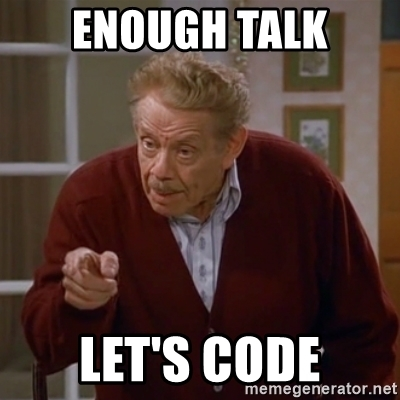
\includegraphics{img/enough-talk-lets-code.jpg}
\caption{letscoce}
\end{figure}

    \subsection{PALABRAS RESERVADAS}\label{palabras-reservadas}

No podemos usar una palabra reservada como nombre de variable, nombre de
función o cualquier otro identificador. Se usan para definir la
\textbf{sintaxis} y la \textbf{estructura} del lenguaje Python.

En Python, las palabras clave distinguen entre mayúsculas y minúsculas.
Hay 33 palabras clave en Python 3.3. Este número puede variar
ligeramente en el transcurso del tiempo.

\begin{verbatim}
  <th></th>
  <th></th>
  <th></th>
  <th></th>
  <th></th>
\end{verbatim}

\begin{verbatim}
<td>False</td>
<td>class</td> 
<td>finally</td>
<td>is</td>
<td>return</td>
\end{verbatim}

\begin{verbatim}
<td>None</td>
<td>continue</td> 
<td>for</td>
<td>lambda</td>
<td>try</td>
\end{verbatim}

\begin{verbatim}
<td>True</td>
<td>def</td> 
<td>from</td>
<td>nonlocal</td>
<td>while</td>
\end{verbatim}

\begin{verbatim}
<td>and</td>
<td>del</td> 
<td>global</td>
<td>not</td>
<td>with</td>
\end{verbatim}

\begin{verbatim}
<td>as</td>
<td>elif</td> 
<td>if</td>
<td>or</td>
<td>yield</td>
\end{verbatim}

\begin{verbatim}
<td>assert</td>
<td>else</td> 
<td>import</td>
<td>pass</td>
<td></td>
\end{verbatim}

\begin{verbatim}
<td>break</td>
<td>except</td> 
<td>in</td>
<td>raise</td>
<td></td>
\end{verbatim}

Si quieres ver un ejemplo de como se usan estas palabras reservadas, te
dejo este link

    \subsection{IDENTIFICADORES}\label{identificadores}

Identificadores en Python es el nombre dado a entidades como clase,
funciones, variables, etc. \textbf{Ayudan a diferenciar una entidad de
otra.}

\subsubsection{Reglas para escribir
identificadores}\label{reglas-para-escribir-identificadores}

\begin{verbatim}
<li>Los identificadores pueden ser una **combinación de letras** en minúsculas (a a z) o mayúsculas (A a Z) o **dígitos** (0 a 9) o un **guión bajo** (_). Nombres como myClass, var_1 e print_this_to_screen, todos son ejemplos válidos.</li>
<li>Un identificador no puede comenzar con un dígito. La variable 1 no es válida, pero la variable 1 está perfectamente bien.</li>
<li>Las palabras reservadas no se pueden usar como identificadores.</li>
<li>No puedes usar simbolos especiales como !, @, #, $, %, etc. en un identificador</li>
<li>El identificador puede ser de cualquier longitud.</li>
\end{verbatim}

\subsubsection{Cosas a tener en cuenta}\label{cosas-a-tener-en-cuenta}

\begin{verbatim}
<li>Python es un lenguaje sensible a mayúsculas y minúsculas. Esto significa que `Variable` y `variable` no son lo mismo. Siempre nombra identificadores que tengan sentido.</li>
<li>Mientras que, `c = 10` es válido. Escribir `count = 10` tendría más sentido y sería más fácil averiguar lo que hace, incluso cuando ves su código después de mucho tiempo.</li>
<li>Se pueden separar varias palabras usando un guión bajo, `this_is_a_long_variable`.</li>
<li>También podemos usar el estilo de escritura camel-case, es decir, poner en mayúscula cada primera letra de la palabra excepto la palabra inicial sin espacios. Por ejemplo: `camelCaseExample`</li>
\end{verbatim}

    \begin{Verbatim}[commandchars=\\\{\}]
{\color{incolor}In [{\color{incolor}17}]:} \PY{c+c1}{\PYZsh{}palabra reservada global no se puede usar como identificador}
         \PY{k}{global} \PY{o}{=} \PY{l+m+mi}{1}
\end{Verbatim}


    \begin{Verbatim}[commandchars=\\\{\}]

          File "<ipython-input-17-3d177345d6e4>", line 1
        global = 1
               \^{}
    SyntaxError: invalid syntax
    

    \end{Verbatim}

    \begin{Verbatim}[commandchars=\\\{\}]
{\color{incolor}In [{\color{incolor}19}]:} \PY{c+c1}{\PYZsh{} no puedes usar simbolos especiales en un identificador}
         \PY{n}{a}\PY{o}{@} \PY{o}{=} \PY{l+m+mi}{0}
\end{Verbatim}


    \begin{Verbatim}[commandchars=\\\{\}]

          File "<ipython-input-19-601cfad26617>", line 2
        a@ = 0
           \^{}
    SyntaxError: invalid syntax
    

    \end{Verbatim}

    \subsection{DECLARACIONES (Statement)}\label{declaraciones-statement}

Las \textbf{instrucciones} que un intérprete de \textbf{Python puede
ejecutar} se llaman declaraciones. Por ejemplo, a = 1 es una declaración
de asignación. if statement, for statement, while statement, etc. son
otros tipos de declaraciones que se analizarán más adelante. \#\#\#
Declaración de varias líneas En Python, el final de una declaración está
marcado por un carácter de nueva línea. Pero podemos hacer que una
declaración se extienda sobre múltiples líneas con el carácter de
continuación de línea ().

    \begin{Verbatim}[commandchars=\\\{\}]
{\color{incolor}In [{\color{incolor}21}]:} \PY{n}{a} \PY{o}{=} \PY{l+m+mi}{1} \PY{o}{+} \PY{l+m+mi}{2} \PY{o}{+} \PY{l+m+mi}{3} \PY{o}{+} \PYZbs{}
             \PY{l+m+mi}{4} \PY{o}{+} \PY{l+m+mi}{5} \PY{o}{+} \PY{l+m+mi}{6} \PY{o}{+} \PYZbs{}
             \PY{l+m+mi}{7} \PY{o}{+} \PY{l+m+mi}{8} \PY{o}{+} \PY{l+m+mi}{9}
\end{Verbatim}


    Esto también se puede hacer usando () \{\} {[}{]}

    \begin{Verbatim}[commandchars=\\\{\}]
{\color{incolor}In [{\color{incolor}23}]:} \PY{n}{b} \PY{o}{=} \PY{p}{(}\PY{l+m+mi}{1} \PY{o}{+} \PY{l+m+mi}{2} \PY{o}{+} \PY{l+m+mi}{3} \PY{o}{+}
             \PY{l+m+mi}{4} \PY{o}{+} \PY{l+m+mi}{5} \PY{o}{+} \PY{l+m+mi}{6} \PY{o}{+}
             \PY{l+m+mi}{7} \PY{o}{+} \PY{l+m+mi}{8} \PY{o}{+} \PY{l+m+mi}{9}\PY{p}{)}
         
         \PY{n}{colors} \PY{o}{=} \PY{p}{[}\PY{l+s+s1}{\PYZsq{}}\PY{l+s+s1}{red}\PY{l+s+s1}{\PYZsq{}}\PY{p}{,}
                   \PY{l+s+s1}{\PYZsq{}}\PY{l+s+s1}{blue}\PY{l+s+s1}{\PYZsq{}}\PY{p}{,}
                   \PY{l+s+s1}{\PYZsq{}}\PY{l+s+s1}{green}\PY{l+s+s1}{\PYZsq{}}\PY{p}{]}
\end{Verbatim}


    \subsection{IDENTACIÓN}\label{identaciuxf3n}

La mayoría de los lenguajes de programación como C, C ++, Java usan
llaves \{\} para definir un bloque de código. Python usa identación.

Un bloque de código (cuerpo de una función, ciclo, etc.) comienza con
una identación y termina con la primera línea sin identar. La cantidad
de identación depende de cada uno, pero debe ser constante a lo largo de
ese bloque.

En general, se utilizan cuatro espacios en blanco para la identación.

    \begin{Verbatim}[commandchars=\\\{\}]
{\color{incolor}In [{\color{incolor}24}]:} \PY{c+c1}{\PYZsh{} ejemplo de identación}
         \PY{k}{for} \PY{n}{i} \PY{o+ow}{in} \PY{n+nb}{range}\PY{p}{(}\PY{l+m+mi}{1}\PY{p}{,}\PY{l+m+mi}{11}\PY{p}{)}\PY{p}{:}
             \PY{n+nb}{print}\PY{p}{(}\PY{n}{i}\PY{p}{)}
             \PY{k}{if} \PY{n}{i} \PY{o}{==} \PY{l+m+mi}{5}\PY{p}{:}
                 \PY{k}{break}
\end{Verbatim}


    \begin{Verbatim}[commandchars=\\\{\}]
1
2
3
4
5

    \end{Verbatim}

    \subsection{VARIABLES Y CONSTANTES}\label{variables-y-constantes}

\subsubsection{Variable}\label{variable}

En la mayoría de los lenguajes de programación, una variable es
\textbf{una ubicación con nombre} utilizada para \textbf{almacenar datos
en la memoria}. Cada variable debe tener un nombre único llamado
identificador. Es útil pensar en las variables como
\textbf{contenedores} que contienen datos que pueden cambiarse más
adelante durante la programación.

\paragraph{Declarando variables}\label{declarando-variables}

En Python, las variables no necesitan declaración para reservar espacio
de memoria. La "declaración de variable" o "inicialización de variable"
ocurre automáticamente cuando asignamos un valor a una variable.
\#\#\#\# Asignando valor a una variable Puede usar el operador de
asignación \texttt{=} para asignar el valor a una variable.

    \begin{Verbatim}[commandchars=\\\{\}]
{\color{incolor}In [{\color{incolor}25}]:} \PY{n}{website} \PY{o}{=} \PY{l+s+s2}{\PYZdq{}}\PY{l+s+s2}{Apple.com}\PY{l+s+s2}{\PYZdq{}}
         \PY{n+nb}{print}\PY{p}{(}\PY{n}{website}\PY{p}{)}
\end{Verbatim}


    \begin{Verbatim}[commandchars=\\\{\}]
Apple.com

    \end{Verbatim}

    \begin{Verbatim}[commandchars=\\\{\}]
{\color{incolor}In [{\color{incolor}26}]:} \PY{c+c1}{\PYZsh{} se puede asignar multiples valores a multiples variables}
         \PY{n}{a}\PY{p}{,} \PY{n}{b}\PY{p}{,} \PY{n}{c} \PY{o}{=} \PY{l+m+mi}{5}\PY{p}{,} \PY{l+m+mf}{3.2}\PY{p}{,} \PY{l+s+s2}{\PYZdq{}}\PY{l+s+s2}{Hello}\PY{l+s+s2}{\PYZdq{}}
         \PY{n+nb}{print} \PY{p}{(}\PY{n}{a}\PY{p}{)}
         \PY{n+nb}{print} \PY{p}{(}\PY{n}{b}\PY{p}{)}
         \PY{n+nb}{print} \PY{p}{(}\PY{n}{c}\PY{p}{)}
\end{Verbatim}


    \begin{Verbatim}[commandchars=\\\{\}]
5
3.2
Hello

    \end{Verbatim}

    \begin{Verbatim}[commandchars=\\\{\}]
{\color{incolor}In [{\color{incolor}27}]:} \PY{c+c1}{\PYZsh{} asignar el mismo valor a diferentes variables}
         \PY{n}{x} \PY{o}{=} \PY{n}{y} \PY{o}{=} \PY{n}{z} \PY{o}{=} \PY{l+s+s2}{\PYZdq{}}\PY{l+s+s2}{same}\PY{l+s+s2}{\PYZdq{}}
         
         \PY{n+nb}{print} \PY{p}{(}\PY{n}{x}\PY{p}{)}
         \PY{n+nb}{print} \PY{p}{(}\PY{n}{y}\PY{p}{)}
         \PY{n+nb}{print} \PY{p}{(}\PY{n}{z}\PY{p}{)}
\end{Verbatim}


    \begin{Verbatim}[commandchars=\\\{\}]
same
same
same

    \end{Verbatim}

    \subsubsection{Constante}\label{constante}

Una constante es un tipo de variable cuyo valor no se puede cambiar. Es
útil pensar en constantes como contenedores que contienen información
que no se puede cambiar más adelante. Deben ser declaradas en mayusculas
siempre.

    \begin{Verbatim}[commandchars=\\\{\}]
{\color{incolor}In [{\color{incolor}28}]:} \PY{c+c1}{\PYZsh{} declarar una constante}
         \PY{n}{PI} \PY{o}{=} \PY{l+m+mf}{3.14}
         \PY{n}{GRAVITY} \PY{o}{=} \PY{l+m+mf}{9.8}
\end{Verbatim}


    \subsection{TIPOS DE DATOS}\label{tipos-de-datos}

\subsubsection{Números}\label{nuxfameros}

Los \textbf{enteros}, los números \textbf{flotantes} y los números
\textbf{complejos} pertenecen a la categoría de números Python. Se
definen como clase \texttt{int}, \texttt{float} y \texttt{complex} en
Python.

Podemos usar la función \texttt{type()} para saber a qué clase pertenece
una variable o un valor y la función \texttt{isinstance()} para
verificar si un objeto pertenece a una clase en particular.

    \begin{Verbatim}[commandchars=\\\{\}]
{\color{incolor}In [{\color{incolor}15}]:} \PY{n}{a} \PY{o}{=} \PY{l+m+mi}{5}
         \PY{n+nb}{print}\PY{p}{(}\PY{n}{a}\PY{p}{,} \PY{l+s+s2}{\PYZdq{}}\PY{l+s+s2}{is of type}\PY{l+s+s2}{\PYZdq{}}\PY{p}{,} \PY{n+nb}{type}\PY{p}{(}\PY{n}{a}\PY{p}{)}\PY{p}{)}
         
         \PY{n}{a} \PY{o}{=} \PY{l+m+mf}{2.0}
         \PY{n+nb}{print}\PY{p}{(}\PY{n}{a}\PY{p}{,} \PY{l+s+s2}{\PYZdq{}}\PY{l+s+s2}{is of type}\PY{l+s+s2}{\PYZdq{}}\PY{p}{,} \PY{n+nb}{type}\PY{p}{(}\PY{n}{a}\PY{p}{)}\PY{p}{)}
         
         \PY{n}{a} \PY{o}{=} \PY{l+m+mi}{1}\PY{o}{+}\PY{l+m+mi}{2}\PY{n}{j}
         \PY{n+nb}{print}\PY{p}{(}\PY{n}{a}\PY{p}{,} \PY{l+s+s2}{\PYZdq{}}\PY{l+s+s2}{is complex number?}\PY{l+s+s2}{\PYZdq{}}\PY{p}{,} \PY{n+nb}{isinstance}\PY{p}{(}\PY{l+m+mi}{1}\PY{o}{+}\PY{l+m+mi}{2}\PY{n}{j}\PY{p}{,}\PY{n+nb}{complex}\PY{p}{)}\PY{p}{)}
\end{Verbatim}


    \begin{Verbatim}[commandchars=\\\{\}]
5 is of type <class 'int'>
2.0 is of type <class 'float'>
(1+2j) is complex number? True

    \end{Verbatim}

    Los \textbf{enteros} pueden ser de cualquier longitud, solo están
limitados por la memoria disponible.

Un \textbf{número de punto flotante} es exacto hasta 15 decimales. Los
puntos enteros y flotantes están separados por puntos decimales.
\texttt{1} es un número entero, \texttt{1.0} es un número de punto
flotante.

Los \textbf{números complejos} se escriben en la forma,
\texttt{x\ +\ yj}, donde \texttt{x} es la parte real e \texttt{y} es la
parte imaginaria.

    \subsubsection{Lista (List)}\label{lista-list}

La lista es una \textbf{secuencia ordenada de elementos}. Es uno de los
tipos de datos más utilizados en Python y es muy flexible. Todos los
elementos en una lista no necesitan ser del mismo tipo.

Declarar una lista es bastante directo. Los elementos separados por
comas se incluyen entre corchetes \texttt{{[}{]}}.

\texttt{a\ =\ {[}1,\ 2.2,\ \textquotesingle{}python\textquotesingle{}{]}}

Podemos usar el operador de división \texttt{{[}{]}} para extraer un
elemento o un rango de elementos de una lista. El índice comienza la
forma 0 en Python.

    \begin{Verbatim}[commandchars=\\\{\}]
{\color{incolor}In [{\color{incolor}29}]:} \PY{n}{a} \PY{o}{=} \PY{p}{[}\PY{l+m+mi}{5}\PY{p}{,}\PY{l+m+mi}{10}\PY{p}{,}\PY{l+m+mi}{15}\PY{p}{,}\PY{l+m+mi}{20}\PY{p}{,}\PY{l+m+mi}{25}\PY{p}{,}\PY{l+m+mi}{30}\PY{p}{,}\PY{l+m+mi}{35}\PY{p}{,}\PY{l+m+mi}{40}\PY{p}{]}
         
         \PY{c+c1}{\PYZsh{} a[2] = 15}
         \PY{n+nb}{print}\PY{p}{(}\PY{l+s+s2}{\PYZdq{}}\PY{l+s+s2}{a[2] = }\PY{l+s+s2}{\PYZdq{}}\PY{p}{,} \PY{n}{a}\PY{p}{[}\PY{l+m+mi}{2}\PY{p}{]}\PY{p}{)}
         
         \PY{c+c1}{\PYZsh{} a[0:3] = [5, 10, 15]}
         \PY{n+nb}{print}\PY{p}{(}\PY{l+s+s2}{\PYZdq{}}\PY{l+s+s2}{a[0:3] = }\PY{l+s+s2}{\PYZdq{}}\PY{p}{,} \PY{n}{a}\PY{p}{[}\PY{l+m+mi}{0}\PY{p}{:}\PY{l+m+mi}{3}\PY{p}{]}\PY{p}{)}
         
         \PY{c+c1}{\PYZsh{} a[5:] = [30, 35, 40]}
         \PY{n+nb}{print}\PY{p}{(}\PY{l+s+s2}{\PYZdq{}}\PY{l+s+s2}{a[5:] = }\PY{l+s+s2}{\PYZdq{}}\PY{p}{,} \PY{n}{a}\PY{p}{[}\PY{l+m+mi}{5}\PY{p}{:}\PY{p}{]}\PY{p}{)}
\end{Verbatim}


    \begin{Verbatim}[commandchars=\\\{\}]
a[2] =  15
a[0:3] =  [5, 10, 15]
a[5:] =  [30, 35, 40]

    \end{Verbatim}

    Las listas son mutables, es decir, el valor de los elementos de una
lista puede modificarse.

    \begin{Verbatim}[commandchars=\\\{\}]
{\color{incolor}In [{\color{incolor}30}]:} \PY{n}{a} \PY{o}{=} \PY{p}{[}\PY{l+m+mi}{1}\PY{p}{,}\PY{l+m+mi}{2}\PY{p}{,}\PY{l+m+mi}{3}\PY{p}{]}
         \PY{n}{a}\PY{p}{[}\PY{l+m+mi}{2}\PY{p}{]}\PY{o}{=}\PY{l+m+mi}{4}
         \PY{n}{a}
\end{Verbatim}


\begin{Verbatim}[commandchars=\\\{\}]
{\color{outcolor}Out[{\color{outcolor}30}]:} [1, 2, 4]
\end{Verbatim}
            
    \subsubsection{Tuplas (Tuple)}\label{tuplas-tuple}

Tuple es una \textbf{secuencia ordenada de elementos} igual que la
lista. La única diferencia es que las tuplas son \textbf{inmutables}.
Las tuplas una vez creadas no se pueden modificar.

Las tuplas se usan para \textbf{proteger contra escritura de datos} y
generalmente son más rápidas que la lista, ya que no pueden cambiar
dinámicamente.

Se define entre paréntesis \texttt{()} donde los elementos están
separados por comas.

    \begin{Verbatim}[commandchars=\\\{\}]
{\color{incolor}In [{\color{incolor}32}]:} \PY{n}{t} \PY{o}{=} \PY{p}{(}\PY{l+m+mi}{5}\PY{p}{,}\PY{l+s+s1}{\PYZsq{}}\PY{l+s+s1}{program}\PY{l+s+s1}{\PYZsq{}}\PY{p}{,} \PY{l+m+mi}{1}\PY{o}{+}\PY{l+m+mi}{3}\PY{n}{j}\PY{p}{)}
         \PY{n}{t}
\end{Verbatim}


\begin{Verbatim}[commandchars=\\\{\}]
{\color{outcolor}Out[{\color{outcolor}32}]:} (5, 'program', (1+3j))
\end{Verbatim}
            
    \subsubsection{Cadenas (Strings)}\label{cadenas-strings}

String es una secuencia de caracteres Unicode. Podemos usar comillas
simples o comillas dobles para representar cadenas. Las cadenas de
varias líneas se pueden denotar utilizando comillas triples,
\texttt{\textquotesingle{}\textquotesingle{}\textquotesingle{}} o
\texttt{"""}.

    \begin{Verbatim}[commandchars=\\\{\}]
{\color{incolor}In [{\color{incolor}35}]:} \PY{n}{s} \PY{o}{=} \PY{l+s+s1}{\PYZsq{}}\PY{l+s+s1}{Hello world!}\PY{l+s+s1}{\PYZsq{}}
         
         \PY{c+c1}{\PYZsh{} s[4] = \PYZsq{}o\PYZsq{}}
         \PY{n+nb}{print}\PY{p}{(}\PY{l+s+s2}{\PYZdq{}}\PY{l+s+s2}{s[4] = }\PY{l+s+s2}{\PYZdq{}}\PY{p}{,} \PY{n}{s}\PY{p}{[}\PY{l+m+mi}{4}\PY{p}{]}\PY{p}{)}
\end{Verbatim}


    \begin{Verbatim}[commandchars=\\\{\}]
s[4] =  o

    \end{Verbatim}

    \subsubsection{Set}\label{set}

es una \textbf{colección desordenada} de elementos \textbf{únicos}. Set
está definido por valores separados por comas dentro de llaves
\texttt{\{\}}. Los artículos en un set no están ordenados.

    \begin{Verbatim}[commandchars=\\\{\}]
{\color{incolor}In [{\color{incolor}36}]:} \PY{n}{a} \PY{o}{=} \PY{p}{\PYZob{}}\PY{l+m+mi}{5}\PY{p}{,}\PY{l+m+mi}{2}\PY{p}{,}\PY{l+m+mi}{3}\PY{p}{,}\PY{l+m+mi}{1}\PY{p}{,}\PY{l+m+mi}{4}\PY{p}{\PYZcb{}}
         
         \PY{c+c1}{\PYZsh{} printing set variable}
         \PY{n+nb}{print}\PY{p}{(}\PY{l+s+s2}{\PYZdq{}}\PY{l+s+s2}{a = }\PY{l+s+s2}{\PYZdq{}}\PY{p}{,} \PY{n}{a}\PY{p}{)}
         
         \PY{c+c1}{\PYZsh{} data type of variable a}
         \PY{n+nb}{print}\PY{p}{(}\PY{n+nb}{type}\PY{p}{(}\PY{n}{a}\PY{p}{)}\PY{p}{)}
\end{Verbatim}


    \begin{Verbatim}[commandchars=\\\{\}]
a =  \{1, 2, 3, 4, 5\}
<class 'set'>

    \end{Verbatim}

    Podemos realizar operaciones de conjunto como unión, intersección en dos
conjuntos. Set tiene valores únicos. Eliminan duplicados.

    \begin{Verbatim}[commandchars=\\\{\}]
{\color{incolor}In [{\color{incolor}38}]:} \PY{n}{a} \PY{o}{=} \PY{p}{\PYZob{}}\PY{l+m+mi}{1}\PY{p}{,}\PY{l+m+mi}{2}\PY{p}{,}\PY{l+m+mi}{2}\PY{p}{,}\PY{l+m+mi}{3}\PY{p}{,}\PY{l+m+mi}{3}\PY{p}{,}\PY{l+m+mi}{3}\PY{p}{\PYZcb{}}
         \PY{n}{a}
\end{Verbatim}


\begin{Verbatim}[commandchars=\\\{\}]
{\color{outcolor}Out[{\color{outcolor}38}]:} \{1, 2, 3\}
\end{Verbatim}
            
    \subsubsection{Diccionario (Dictionary)}\label{diccionario-dictionary}

El diccionario es una \textbf{colección desordenada} de pares
clave-valor.

Generalmente se usa cuando tenemos una \textbf{gran cantidad de datos}.
Los diccionarios están optimizados para recuperar datos. Debemos conocer
la clave para recuperar el valor.

En Python, los diccionarios \textbf{se definen entre llaves}
\texttt{\{\}} con cada elemento siendo un par en la clave de formulario:
valor. La clave y el valor pueden ser de cualquier tipo.

    \begin{Verbatim}[commandchars=\\\{\}]
{\color{incolor}In [{\color{incolor}44}]:} \PY{n}{d} \PY{o}{=} \PY{p}{\PYZob{}}\PY{l+m+mi}{1}\PY{p}{:}\PY{l+s+s1}{\PYZsq{}}\PY{l+s+s1}{value}\PY{l+s+s1}{\PYZsq{}}\PY{p}{,}\PY{l+s+s1}{\PYZsq{}}\PY{l+s+s1}{key}\PY{l+s+s1}{\PYZsq{}}\PY{p}{:}\PY{l+m+mi}{2}\PY{p}{\PYZcb{}}
         \PY{n+nb}{type}\PY{p}{(}\PY{n}{d}\PY{p}{)}
         \PY{n+nb}{print}\PY{p}{(}\PY{l+s+s2}{\PYZdq{}}\PY{l+s+s2}{d[1] = }\PY{l+s+s2}{\PYZdq{}}\PY{p}{,} \PY{n}{d}\PY{p}{[}\PY{l+m+mi}{1}\PY{p}{]}\PY{p}{)}\PY{p}{;}
         
         \PY{n+nb}{print}\PY{p}{(}\PY{l+s+s2}{\PYZdq{}}\PY{l+s+s2}{d[}\PY{l+s+s2}{\PYZsq{}}\PY{l+s+s2}{key}\PY{l+s+s2}{\PYZsq{}}\PY{l+s+s2}{] = }\PY{l+s+s2}{\PYZdq{}}\PY{p}{,} \PY{n}{d}\PY{p}{[}\PY{l+s+s1}{\PYZsq{}}\PY{l+s+s1}{key}\PY{l+s+s1}{\PYZsq{}}\PY{p}{]}\PY{p}{)}\PY{p}{;}
\end{Verbatim}


    \begin{Verbatim}[commandchars=\\\{\}]
d[1] =  value
d['key'] =  2

    \end{Verbatim}

    \subsection{OPERADORES}\label{operadores}

Los operadores son símbolos especiales en Python que realizan cálculos
aritméticos o lógicos. El valor que opera el operador se llama operando.

\subsubsection{Operadores aritméticos}\label{operadores-aritmuxe9ticos}

\begin{verbatim}
<thead>
    <tr>
        <th>Operador</th>
        <th>Significado</th>
        <th>Ejemplo</th>
    </tr>
</thead>
<tbody>
    <tr>
        <td>`+`</td>
        <td>suma</td>
        <td>x + y + 2</td>
    </tr>
    <tr>
        <td>`-`</td>
        <td>resta</td>
        <td>x - y - 2</td>
    </tr>
    <tr>
        <td>`*`</td>
        <td>multiplicación</td>
        <td>x `*` y</td>
    </tr>
    <tr>
        <td>`/`</td>
        <td>división</td>
        <td>x `/` y</td>
    </tr>
    <tr>
        <td>`%`</td>
        <td>modulo - resto de la división de un número por otro</td>
        <td>x `%` y</td>
    </tr>
     <tr>
        <td>`//`</td>
        <td>Cociente de una división - El resultado es siempre un número entero</td>
        <td>x `//` y</td>
    </tr>
     <tr>
        <td>`**`</td>
        <td>Potencia</td>
        <td>x `**` y</td>
    </tr>
</tbody>
\end{verbatim}

    \begin{Verbatim}[commandchars=\\\{\}]
{\color{incolor}In [{\color{incolor}49}]:} \PY{n}{x} \PY{o}{=} \PY{l+m+mi}{15}
         \PY{n}{y} \PY{o}{=} \PY{l+m+mi}{4}
         
         \PY{n+nb}{print}\PY{p}{(}\PY{l+s+s1}{\PYZsq{}}\PY{l+s+s1}{x + y =}\PY{l+s+s1}{\PYZsq{}}\PY{p}{,}\PY{n}{x}\PY{o}{+}\PY{n}{y}\PY{p}{)}
         \PY{n+nb}{print}\PY{p}{(}\PY{l+s+s1}{\PYZsq{}}\PY{l+s+s1}{x \PYZhy{} y =}\PY{l+s+s1}{\PYZsq{}}\PY{p}{,}\PY{n}{x}\PY{o}{\PYZhy{}}\PY{n}{y}\PY{p}{)}
         \PY{n+nb}{print}\PY{p}{(}\PY{l+s+s1}{\PYZsq{}}\PY{l+s+s1}{x * y =}\PY{l+s+s1}{\PYZsq{}}\PY{p}{,}\PY{n}{x}\PY{o}{*}\PY{n}{y}\PY{p}{)}
         \PY{n+nb}{print}\PY{p}{(}\PY{l+s+s1}{\PYZsq{}}\PY{l+s+s1}{x / y =}\PY{l+s+s1}{\PYZsq{}}\PY{p}{,}\PY{n}{x}\PY{o}{/}\PY{n}{y}\PY{p}{)}
         \PY{n+nb}{print}\PY{p}{(}\PY{l+s+s1}{\PYZsq{}}\PY{l+s+s1}{x // y =}\PY{l+s+s1}{\PYZsq{}}\PY{p}{,}\PY{n}{x}\PY{o}{/}\PY{o}{/}\PY{n}{y}\PY{p}{)}
         \PY{n+nb}{print}\PY{p}{(}\PY{l+s+s1}{\PYZsq{}}\PY{l+s+s1}{x ** y =}\PY{l+s+s1}{\PYZsq{}}\PY{p}{,}\PY{n}{x}\PY{o}{*}\PY{o}{*}\PY{n}{y}\PY{p}{)}
\end{Verbatim}


    \begin{Verbatim}[commandchars=\\\{\}]
x + y = 19
x - y = 11
x * y = 60
x / y = 3.75
x // y = 3
x ** y = 50625

    \end{Verbatim}

    \subsubsection{Operadores de
comparación}\label{operadores-de-comparaciuxf3n}

Los operadores de comparación se usan para comparar valores. Devuelve
\texttt{True} o \texttt{False} según la condición.

\begin{verbatim}
<thead>
    <tr>
        <th>Operador</th>
        <th>Significado</th>
        <th>Ejemplo</th>
    </tr>
</thead>
<tbody>
    <tr>
        <td>`>`</td>
        <td>mayor que</td>
        <td>x > y</td>
    </tr>
    <tr>
        <td>`<`</td>
        <td>menor que</td>
        <td>x < y</td>
    </tr>
    <tr>
        <td>`==`</td>
        <td>igual</td>
        <td>x = y</td>
    </tr>
    <tr>
        <td>`!=`</td>
        <td>diferente</td>
        <td>x != y</td>
    </tr>
    <tr>
        <td>`>=`</td>
        <td>mayor igual</td>
        <td>x `>=` y</td>
    </tr>
     <tr>
        <td>`<=`</td>
        <td>menor igual</td>
        <td>x `<=` y</td>
    </tr>
</tbody>
\end{verbatim}

    \begin{Verbatim}[commandchars=\\\{\}]
{\color{incolor}In [{\color{incolor}50}]:} \PY{n}{x} \PY{o}{=} \PY{l+m+mi}{10}
         \PY{n}{y} \PY{o}{=} \PY{l+m+mi}{12}
         
         \PY{n+nb}{print}\PY{p}{(}\PY{l+s+s1}{\PYZsq{}}\PY{l+s+s1}{x \PYZgt{} y  is}\PY{l+s+s1}{\PYZsq{}}\PY{p}{,}\PY{n}{x}\PY{o}{\PYZgt{}}\PY{n}{y}\PY{p}{)}
         \PY{n+nb}{print}\PY{p}{(}\PY{l+s+s1}{\PYZsq{}}\PY{l+s+s1}{x \PYZlt{} y  is}\PY{l+s+s1}{\PYZsq{}}\PY{p}{,}\PY{n}{x}\PY{o}{\PYZlt{}}\PY{n}{y}\PY{p}{)}
         \PY{n+nb}{print}\PY{p}{(}\PY{l+s+s1}{\PYZsq{}}\PY{l+s+s1}{x == y is}\PY{l+s+s1}{\PYZsq{}}\PY{p}{,}\PY{n}{x}\PY{o}{==}\PY{n}{y}\PY{p}{)}
         \PY{n+nb}{print}\PY{p}{(}\PY{l+s+s1}{\PYZsq{}}\PY{l+s+s1}{x != y is}\PY{l+s+s1}{\PYZsq{}}\PY{p}{,}\PY{n}{x}\PY{o}{!=}\PY{n}{y}\PY{p}{)}
         \PY{n+nb}{print}\PY{p}{(}\PY{l+s+s1}{\PYZsq{}}\PY{l+s+s1}{x \PYZgt{}= y is}\PY{l+s+s1}{\PYZsq{}}\PY{p}{,}\PY{n}{x}\PY{o}{\PYZgt{}}\PY{o}{=}\PY{n}{y}\PY{p}{)}
         \PY{n+nb}{print}\PY{p}{(}\PY{l+s+s1}{\PYZsq{}}\PY{l+s+s1}{x \PYZlt{}= y is}\PY{l+s+s1}{\PYZsq{}}\PY{p}{,}\PY{n}{x}\PY{o}{\PYZlt{}}\PY{o}{=}\PY{n}{y}\PY{p}{)}
\end{Verbatim}


    \begin{Verbatim}[commandchars=\\\{\}]
x > y  is False
x < y  is True
x == y is False
x != y is True
x >= y is False
x <= y is True

    \end{Verbatim}

    \subsubsection{Operadores lógicos}\label{operadores-luxf3gicos}

Los operadores lógicos son \texttt{and},\texttt{or}, \texttt{not}.

\paragraph{and}\label{and}

\texttt{and} dará como resultado \texttt{True} solo si ambos operandos
son Verdaderos. La tabla de verdad para \texttt{and} se da a
continuación:

\begin{verbatim}
<thead>
    <tr>
        <th>A</th>
        <th>B</th>
        <th>A and B</th>
    </tr>
</thead>
<tbody>
    <tr>
        <td>True</td>
        <td>True</td>
        <td>True</td>
    </tr>
    <tr>
        <td>True</td>
        <td>False</td>
        <td>False</td>
    </tr>
    <tr>
        <td>False</td>
        <td>True</td>
        <td>False</td>
    </tr>
    <tr>
        <td>False</td>
        <td>False</td>
        <td>False</td>
    </tr>
</tbody>
\end{verbatim}

\paragraph{or}\label{or}

\texttt{or} dará como resultado \texttt{True} solo si alguno de los
operandos son Verdaderos. La tabla de verdad para \texttt{or} se da a
continuación:

\begin{verbatim}
<thead>
    <tr>
        <th>A</th>
        <th>B</th>
        <th>A and B</th>
    </tr>
</thead>
<tbody>
    <tr>
        <td>True</td>
        <td>True</td>
        <td>True</td>
    </tr>
    <tr>
        <td>True</td>
        <td>False</td>
        <td>True</td>
    </tr>
    <tr>
        <td>False</td>
        <td>True</td>
        <td>True</td>
    </tr>
    <tr>
        <td>False</td>
        <td>False</td>
        <td>False</td>
    </tr>
</tbody>
\end{verbatim}

\paragraph{not}\label{not}

\texttt{not} dará como resultado \texttt{True} solo si alguno de los
operandos son Verdaderos. La tabla de verdad para \texttt{or} se da a
continuación:

\begin{verbatim}
<thead>
    <tr>
        <th>A</th>
        <th>not A</th>
    </tr>
</thead>
<tbody>
    <tr>
        <td>True</td>
        <td>False</td>
    </tr>
    <tr>
        <td>False</td>
        <td>True</td>
    </tr>
</tbody>
\end{verbatim}

    \begin{Verbatim}[commandchars=\\\{\}]
{\color{incolor}In [{\color{incolor}58}]:} \PY{k+kc}{True} \PY{o+ow}{and} \PY{k+kc}{False}
         \PY{c+c1}{\PYZsh{}tambien se puede escribir True \PYZam{} False}
\end{Verbatim}


\begin{Verbatim}[commandchars=\\\{\}]
{\color{outcolor}Out[{\color{outcolor}58}]:} False
\end{Verbatim}
            
    \begin{Verbatim}[commandchars=\\\{\}]
{\color{incolor}In [{\color{incolor}60}]:} \PY{k+kc}{True} \PY{o+ow}{or} \PY{k+kc}{False}
         \PY{c+c1}{\PYZsh{} True | False}
\end{Verbatim}


\begin{Verbatim}[commandchars=\\\{\}]
{\color{outcolor}Out[{\color{outcolor}60}]:} True
\end{Verbatim}
            
    \begin{Verbatim}[commandchars=\\\{\}]
{\color{incolor}In [{\color{incolor}63}]:} \PY{o+ow}{not} \PY{k+kc}{False}
\end{Verbatim}


\begin{Verbatim}[commandchars=\\\{\}]
{\color{outcolor}Out[{\color{outcolor}63}]:} True
\end{Verbatim}
            
    \subsubsection{Operadores de
asignación}\label{operadores-de-asignaciuxf3n}

Los operadores de asignación se usan en Python para asignar valores a
las variables.

\begin{verbatim}
<thead>
    <tr>
        <th>Operador</th>
        <th>ejemplo</th>
        <th>Equivalente a</th>
    </tr>
</thead>
<tbody>
    <tr>
        <td>`=`</td>
        <td>`x=5`</td>
        <td>`x = 5`</td>
    </tr>
    <tr>
        <td>`+=`</td>
        <td>`x+=5`</td>
        <td>`x = x +5`</td>
    </tr>
    <tr>
        <td>`-=`</td>
        <td>`x-=5`</td>
        <td>`x = x -5`</td>
    </tr>
    <tr>
        <td>`*=`</td>
        <td>`x*=5`</td>
        <td>`x = x*5`</td>
    </tr>
</tbody>
\end{verbatim}

    \subsection{Operadores de identidad}\label{operadores-de-identidad}

\texttt{is} y \texttt{is\ not} son los operadores de identidad en
Python. Se usan para verificar si dos valores (o variables) se
encuentran en la misma parte de la memoria. Dos variables que son
iguales no implican que sean idénticas.

\begin{verbatim}
<thead>
    <tr>
        <th>Operador</th>
        <th>significado</th>
        <th>ejemplo a</th>
    </tr>
</thead>
<tbody>
    <tr>
        <td>`is`</td>
        <td>True si los operandos son idénticos</td>
        <td>`x is True`</td>
    </tr>
    <tr>
        <td>`is not`</td>
        <td>True si los operandos no son idénticos</td>
        <td>`x is not True`</td>
    </tr>
</tbody>
\end{verbatim}

    \begin{Verbatim}[commandchars=\\\{\}]
{\color{incolor}In [{\color{incolor}65}]:} \PY{n}{x1} \PY{o}{=} \PY{l+m+mi}{5}
         \PY{n}{y1} \PY{o}{=} \PY{l+m+mi}{5}
         \PY{n}{x2} \PY{o}{=} \PY{l+s+s1}{\PYZsq{}}\PY{l+s+s1}{Hello}\PY{l+s+s1}{\PYZsq{}}
         \PY{n}{y2} \PY{o}{=} \PY{l+s+s1}{\PYZsq{}}\PY{l+s+s1}{Hello}\PY{l+s+s1}{\PYZsq{}}
         \PY{n}{x3} \PY{o}{=} \PY{p}{[}\PY{l+m+mi}{1}\PY{p}{,}\PY{l+m+mi}{2}\PY{p}{,}\PY{l+m+mi}{3}\PY{p}{]}
         \PY{n}{y3} \PY{o}{=} \PY{p}{[}\PY{l+m+mi}{1}\PY{p}{,}\PY{l+m+mi}{2}\PY{p}{,}\PY{l+m+mi}{3}\PY{p}{]}
         
         \PY{n+nb}{print}\PY{p}{(}\PY{n}{x1} \PY{o+ow}{is} \PY{o+ow}{not} \PY{n}{y1}\PY{p}{)}
         
         \PY{n+nb}{print}\PY{p}{(}\PY{n}{x2} \PY{o+ow}{is} \PY{n}{y2}\PY{p}{)}
         
         \PY{n+nb}{print}\PY{p}{(}\PY{n}{x3} \PY{o+ow}{is} \PY{n}{y3}\PY{p}{)}
\end{Verbatim}


    \begin{Verbatim}[commandchars=\\\{\}]
False
True
False

    \end{Verbatim}

    \subsubsection{Operadores de pertenecia}\label{operadores-de-pertenecia}

\texttt{in} y \texttt{not\ in} son los operadores de pertenecia en
Python. Se usan para probar si un valor o variable se encuentra en una
secuencia (cadena, lista, tupla, conjunto y diccionario).

\begin{verbatim}
<thead>
    <tr>
        <th>Operador</th>
        <th>significado</th>
        <th>ejemplo a</th>
    </tr>
</thead>
<tbody>
    <tr>
        <td>`in`</td>
        <td>True si la variable o valor se encuentra en la secuencia</td>
        <td>`5 in x`</td>
    </tr>
    <tr>
        <td>`not in`</td>
        <td>True si la variable o valor no se encuentra en la secuencia</td>
        <td>`5 not in x`</td>
    </tr>
</tbody>
\end{verbatim}

    \begin{Verbatim}[commandchars=\\\{\}]
{\color{incolor}In [{\color{incolor}66}]:} \PY{n}{x} \PY{o}{=} \PY{l+s+s1}{\PYZsq{}}\PY{l+s+s1}{Hello world}\PY{l+s+s1}{\PYZsq{}}
         \PY{n}{y} \PY{o}{=} \PY{p}{\PYZob{}}\PY{l+m+mi}{1}\PY{p}{:}\PY{l+s+s1}{\PYZsq{}}\PY{l+s+s1}{a}\PY{l+s+s1}{\PYZsq{}}\PY{p}{,}\PY{l+m+mi}{2}\PY{p}{:}\PY{l+s+s1}{\PYZsq{}}\PY{l+s+s1}{b}\PY{l+s+s1}{\PYZsq{}}\PY{p}{\PYZcb{}}
         
         \PY{n+nb}{print}\PY{p}{(}\PY{l+s+s1}{\PYZsq{}}\PY{l+s+s1}{H}\PY{l+s+s1}{\PYZsq{}} \PY{o+ow}{in} \PY{n}{x}\PY{p}{)}
         
         \PY{n+nb}{print}\PY{p}{(}\PY{l+s+s1}{\PYZsq{}}\PY{l+s+s1}{hello}\PY{l+s+s1}{\PYZsq{}} \PY{o+ow}{not} \PY{o+ow}{in} \PY{n}{x}\PY{p}{)}
         
         \PY{n+nb}{print}\PY{p}{(}\PY{l+m+mi}{1} \PY{o+ow}{in} \PY{n}{y}\PY{p}{)}
         
         \PY{n+nb}{print}\PY{p}{(}\PY{l+s+s1}{\PYZsq{}}\PY{l+s+s1}{a}\PY{l+s+s1}{\PYZsq{}} \PY{o+ow}{in} \PY{n}{y}\PY{p}{)}
\end{Verbatim}


    \begin{Verbatim}[commandchars=\\\{\}]
True
True
True
False

    \end{Verbatim}


    % Add a bibliography block to the postdoc
    
    
    
    \end{document}
